\section{Overview of the Approach}

The key objective of our SLA compliance monitoring system presented in this paper is fast deployment in an environment in which the subject of monitoring is evolving quickly and services expose a variety of measurement interfaces. This section provides an overview of our approach how to address those issues at the same time. The first subsection discusses the system model outlining how the rSLA service interacts with interfaces of a heterogeneous environment. The second part outlines the major elements of an SLA document's content.

\subsection{System Model}

Cost, availability and on-demand scaling have accelerated customer adoption of different application deployment models - On-Premise cloud, Private cloud, Public cloud or hybrid 
clouds, in addition to their traditional dedicated environments. Depending on the services that an application depends on, the choice of platform varies. A single application could potentially be reliant on multiple clouds for the set of 
services it consumes. From a customer/tenant perspective, monitoring service levels that their workloads are getting often becomes a complex task of aggregating information across 
multiple cloud providers, each using different proprietary monitoring and management stacks. Further aggravating the problem is the devops transition. Applications and consequently 
their bindings to services are seeing an increased rate of change. 

\begin{figure}[H]
\centering
 \includegraphics[width=8cm,height=8cm]{pics/systemModel.pdf} 
 \caption{rSLA System Overview}
 \label{fig:systemModel}
\end{figure}

Figure \ref{fig:systemModel} shows an overview of the proposed rSLA system model. The rSLA framework is made up three main components:
\begin{enumerate}
\item a language for administrators or service providers to express service level agreements; 
\item a set of  Xlets - lightweight, dynamically bound adapters; xlets abstract the heterogeneity of service management interfaces to rSLA, both for the reading of metrics as well as the acting on the result of SLA evaluation; and
\item a modular SLA evaluation service; this service interprets the rSLA document. It performs the reading of measurements through monitoring xlets as defined in the document, aggregates metrics, evaluated compliance and then notifies stakeholders.
\end{enumerate}

A formal language for SLAs is the key to both custom SLAs on a case-by-case basis and fast deployment of the SLA. The xlet approach provides the level of abstraction and indirection to intermediate between service interface heterogeneity and the need of the SLA evaluation service to read metrics in a homogenous way. 

The rSLA evaluation itself can be deployed in any 
of the cloud deployment models - On-Premise cloud, Private cloud, Public cloud or hybrid clouds. Further sections describe the language concepts, the execution model, and implementation. The case study discusses some xlets we wrote for a particular Cloud service.



